\pgfsetplotmarksize{0pt}
\begin{figure}
 \centering
 \caption{\label{fl_conv8}UflLib/Euclid/111EuclS.txt},
 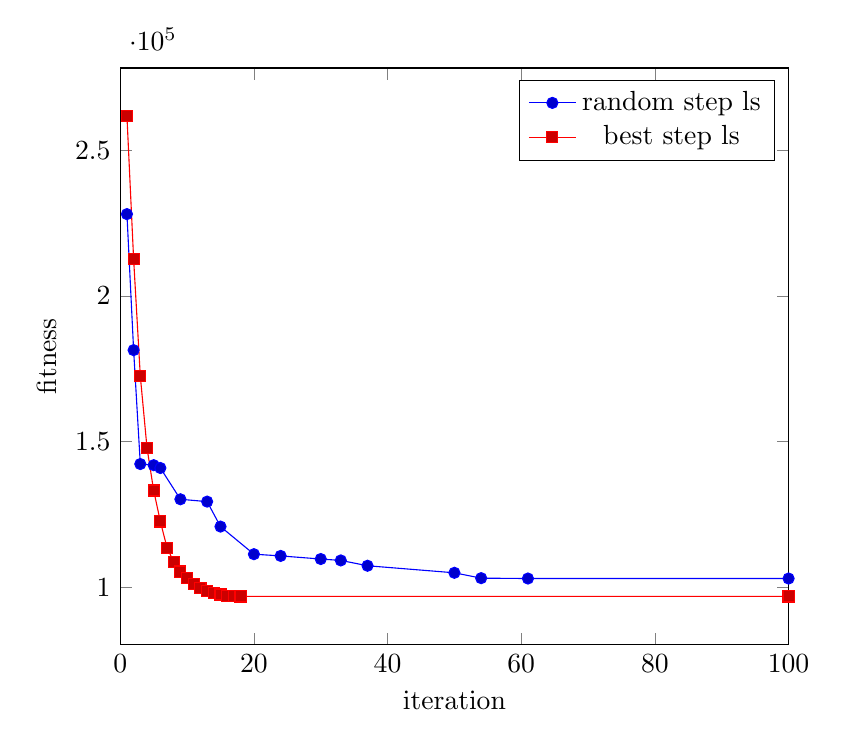
\begin{tikzpicture}
 \begin{axis}[
   width=0.7\textwidth,
   scale only axis,
   xlabel=iteration,
   ylabel=fitness,
   xmin=0,xmax=100,
   domain=0:100]
   \addplot coordinates {
     (0,inf)
     (1,228070)
     (2,181382)
     (3,142280)
     (5,141889)
     (6,140923)
     (9,130182)
     (13,129380)
     (15,120806)
     (20,111336)
     (24,110742)
     (30,109671)
     (33,109190)
     (37,107363)
     (50,104944)
     (54,103108)
     (61,102980)
     (100,102980)
   };
   \addlegendentry{random step ls}
   \addplot coordinates {
     (0,inf)
     (1,261723)
     (2,212629)
     (3,172510)
     (4,147871)
     (5,133201)
     (6,122566)
     (7,113550)
     (8,108730)
     (9,105367)
     (10,103084)
     (11,101058)
     (12,99660)
     (13,98707)
     (14,97950)
     (15,97497)
     (16,97106)
     (17,96929)
     (18,96831)
     (100,96831)
   };
   \addlegendentry{best step ls}
 \end{axis}
 \end{tikzpicture}
\end{figure}
